
\chapter{3D Molecular Dynamics Results and Comparison with Experimental Data}

The 3D molecular dynamics simulation was run for $\SI{100}{\nano\second}$ at $\SI{140}{\kelvin}$ using the Morse parameters in Table \ref{table:fit_parameters} and a $20\times20\times20$ substrate. The results of this simulation are summarized in Figure \ref{fig:md_results}.

\section{Discussion and Analysis of ISFs}

Figures \ref{fig:md_isf_0.6} \& \ref{fig:md_isf_1.2} show the simulated ISFs in the $\left[11\bar{2}\right]$ direction overlayed with experimental HSEM data\footnote{The experimental data is shown as black crosses. The red, green and blue lines were included in the results in \cite{Ward} but may be ignored for the purposes of this report.\label{rgb_lines}} taken from \cite{Ward}. At very short times, $t \sim \SI{e-1}{\pico\second}$, we see agreement of the experimental data and the MD simulation. The Gaussian shape of the ISF at this very short timescale is driven by ballistic motion solely parameterized by the 2D thermal velocity of the lithium, $v=\sqrt{\frac{2k_BT}{m}}$ \cite{Ward}. Experimental results have shown that the effective mass of lithium on copper is equal to its atomic mass so this result is expected \cite{Ward}. 

At long times, the simulated ISFs are found to decay much faster than the experimental ones. Since the simulation was setup with a hopping potential barrier similar to the experimentally determined value, this classical simulation fails to capture the pre-exponential factor of the real system. 

The molecular dynamics simulation disagrees with experimental data on the relative contributions of fast to slow motion in the ISF. This is apparent in the proportion of the ISF's drop off which occurs in the first few picoseconds relative to the slow decay. Previous work on lithium on copper(111) has explained similar discrepancies by introducing GLE simulations with a band limited noise spectrum \cite{Ward}. However, the frequency cutoff required was found to be almost an order of magnitude lower than the phonon cutoff frequency in copper. This explains why the MD simulation, is unable to reproduce this aspect of the experimental data.

Figure \ref{fig:isf_0.6_dkz_included} is indicative of the additional structure in the ISF which is missed by the Cambridge HSEM apparatus due to insensitivity to the very high frequency components of the signal. In light of the discussion in Chapter \ref{sec:gle_interpretation}, these oscillations may be used to extract useful information about the system in the $\left[111\right]$ direction if they ever become experimentally accessible.

\section{Discussion and Analysis of simulated hopping rates}

Figure \ref{fig:alpha_deltak} shows the dephasing rate of the ISF in the $\left[1\bar{1}0\right]$ direction as a function of $\Delta{\vec{K}}$. As pointed out in \cite{TUDDENHAM20101459}, although the fcc 111 surface is not a Bravais lattice and the hops occur between between non-equivalent lattice sites, the ISF in the $\left[1\bar{1}0\right]$ direction is equivalent to a particle hopping on a 1D lattice with half the lattice spacing of the fcc crystal. The ISF of such idealized hopping is given by the Chudley-Elliot model and predicts a dephasing rate of
\\
$$
	\alpha\left(\Delta{K}\right) = 2\Gamma\sin^2\left(\frac{a\Delta{K}}{2}\right)
$$
\\
Where $\alpha$ is the dephasing rate, $\Gamma$ is the hopping rate and $a$ is the equivalent 1D nearest neighbor distance. Figure \ref{fig:alpha_deltak} therefore suggests that the simulation exhibits a hopping rate of $\SI{0.62}{\per\pico\second}$ for hops with a component in the $\left[1\bar{1}0\right]$ direction. Rotational symmetry of the system may then be used to argue that the total hopping rate is approximately $\Gamma_{\text{tot}} = \frac{3}{2}\Gamma = \SI{0.93}{\per\pico\second}$. Therefore the hopping of the system is likely to be sensitive to changes in the Fourier spectrum around $\sim\SI{1}{\tera\hertz}$ or less. Much higher frequencies noise components are unlikely to affect hopping as they average out over the timescale of a picosecond. 

Figure \ref{fig:ahrrenius_plot} Shows the logarithm of the maximum ISF dephasing rate as a function of inverse temperature. The fitting process used to extract the maximum dephasing rate was hindered by phonon oscillations and noise. This introduced a large degree of uncertainty into this estimate even when the Fourier filter method suggested in the \cite{Ward} was used. Nevertheless this results in \ref{fig:ahrrenius_plot} are consistent with an Arrhenius law with activation energy $E_a=9.6\pm\SI{1.5}{\mev}$ and confirm that the pre-exponential factor of the decay rate is not reproduced by MD simulation.

\begin{figure}
	\begin{subfigure}{0.49\textwidth}
		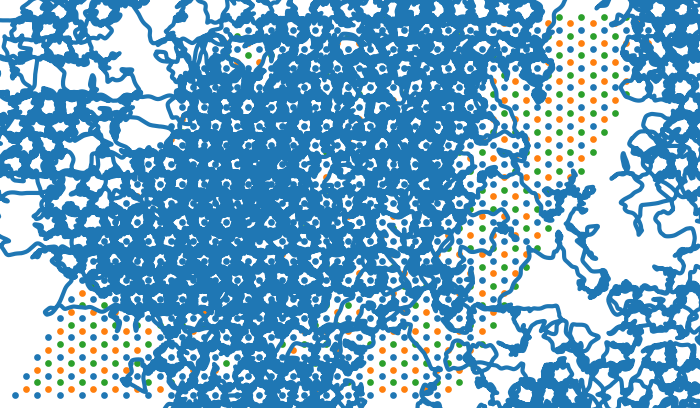
\includegraphics[width=1.0\textwidth]{md_top_down}
		\caption{The trajectory of the adatom overlayed on the equilibrium position of the top 3 substrate layers. Periodic substrate boundary conditions allow the adatom to diffuse outside the bounds of the substrate.}
		\label{fig:md_top_down}
	\end{subfigure}
	\hfill
	\begin{subfigure}{0.49\textwidth}
		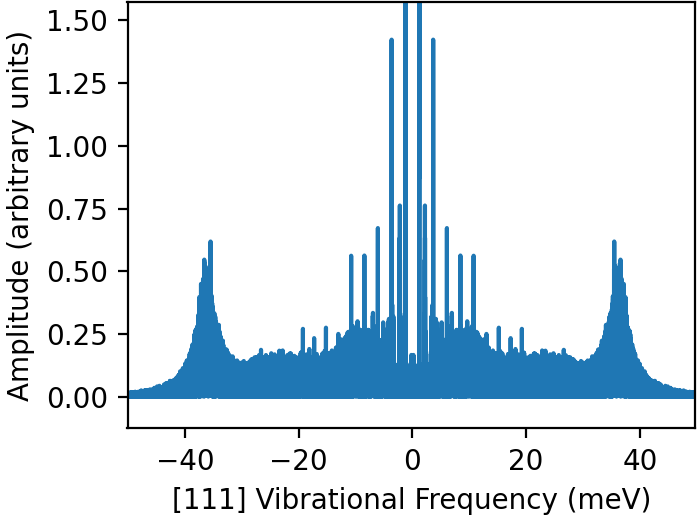
\includegraphics[width=1.0\textwidth]{111_vibrational_fft}
		\caption{The Fourier spectrum of the [111] co-ordinate of the adatom. The peak at $\SI{38}{\mev}$ corresponds to harmonic oscillations around equilibrium as constructed in Section \ref{sec:md_fit}. The phonon cutoff frequency determined in Section \ref{sec:phonon_spectrum} of $\SI{7.4}{\tera\hertz}$ ($\SI{30.5}{\mev}$) is visible but overlaps with the harmonic peak.}
		\label{fig:111_vibrational_fft}
	\end{subfigure}
	
	\begin{subfigure}{0.49\textwidth}
		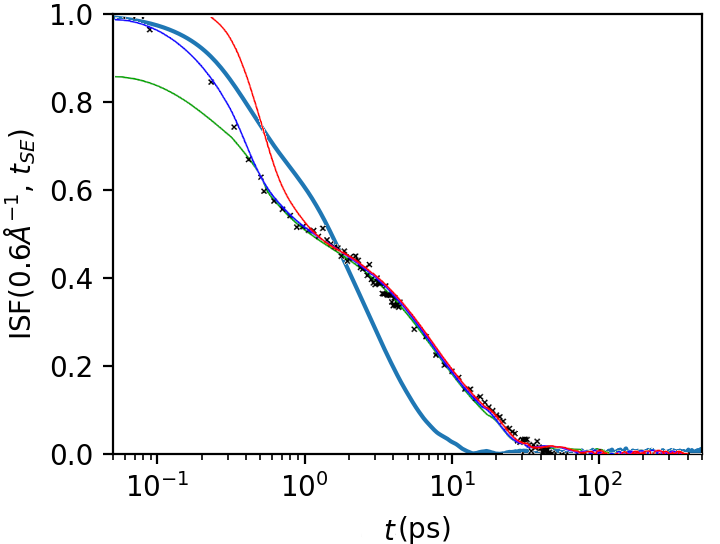
\includegraphics[width=1.0\textwidth]{md_isf_0.6_overlayed}
		\caption{The ISF of the adatom in the $\left[11\bar{2}\right]$ direction with $\left|\Delta{\vec{K}}\right|=\SI{0.6}{\per\angstrom}$. Overlayed in black crosses is HSEM data taken from \cite{Ward} for Lithium on Copper 111 at $\SI{140}{\kelvin}^{\text{\ref{rgb_lines}}}$.}
		\label{fig:md_isf_0.6}
	\end{subfigure}
	\hfill
	\begin{subfigure}{0.49\textwidth}
		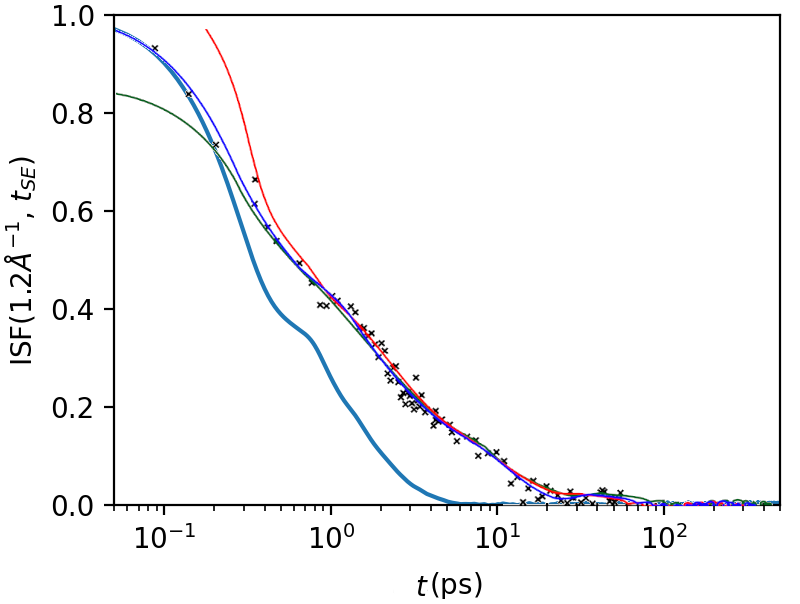
\includegraphics[width=1.0\textwidth]{md_isf_1.2_overlayed}
		\caption{The ISF of the adatom in the $\left[11\bar{2}\right]$ direction with $\left|\Delta{\vec{K}}\right|=\SI{0.6}{\per\angstrom}$. Overlayed in black crosses is HSEM data taken from \cite{Ward} for Lithium on Copper 111 at $\SI{140}{\kelvin}^{\text{\ref{rgb_lines}}}$.}
		\label{fig:md_isf_1.2}
	\end{subfigure}

	\begin{subfigure}{0.49\textwidth}
		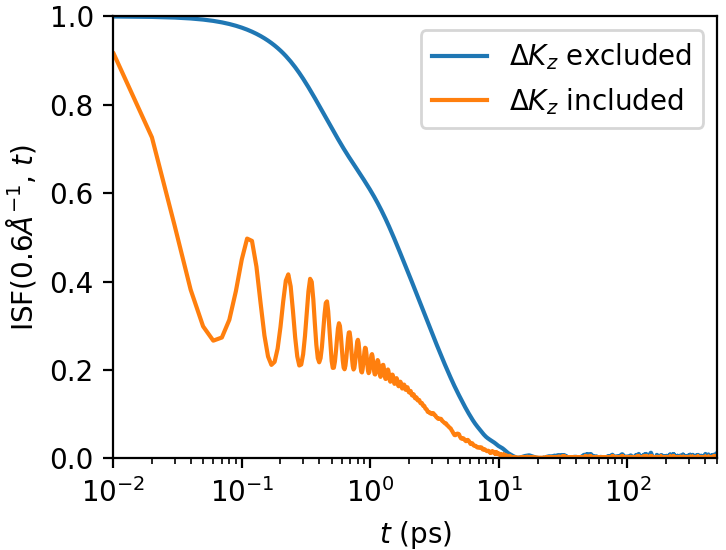
\includegraphics[width=1.0\textwidth]{isf_0.6_dkz_included}
		\caption{Two simulated ISFs with a parallel momentum transfer of $\SI{0.6}{\per\angstrom}$ in the $\left[11\bar{2}\right]$ direction. The momentum transfer used to calculate the orange ISF included an additional z-component of $\SI{9.93}{\per\angstrom}$ consistent with the assumptions of quasi-elastic scattering at the beam energy used in the Cambridge HSEM device \cite{HSEM}.}
		\label{fig:isf_0.6_dkz_included}
	\end{subfigure}
	\hfill
	\begin{subfigure}{0.49\textwidth}
		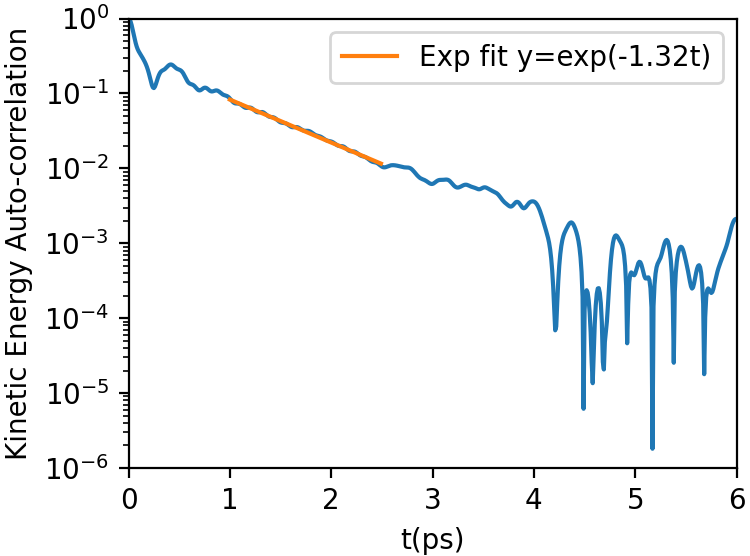
\includegraphics[width=1.0\textwidth]{md_kinetic_energy_autocorrelation}
		\caption{The kinetic energy auto-correlation function of the adatom on a log y-scale. The exponential fit suggests a naive estimate of the friction constant of around $\SI{1.32}{\per\pico\second}$ as per the discussion in Chapter \ref{sec:gle_interpretation}.}
		\label{fig:md_kinetic_energy_autocorrelation}
	\end{subfigure}
	
	\caption{Results of a $\SI{100}{\nano\second}$ run of the 3D molecular dynamics simulation constructed in Section \ref{sec:md_setup} at $\SI{140}{\kelvin}$ with Morse parameters summarized in Table \ref{table:fit_parameters}.}
	\label{fig:md_results}
\end{figure}


\begin{figure}
	\begin{subfigure}{0.49\textwidth}
		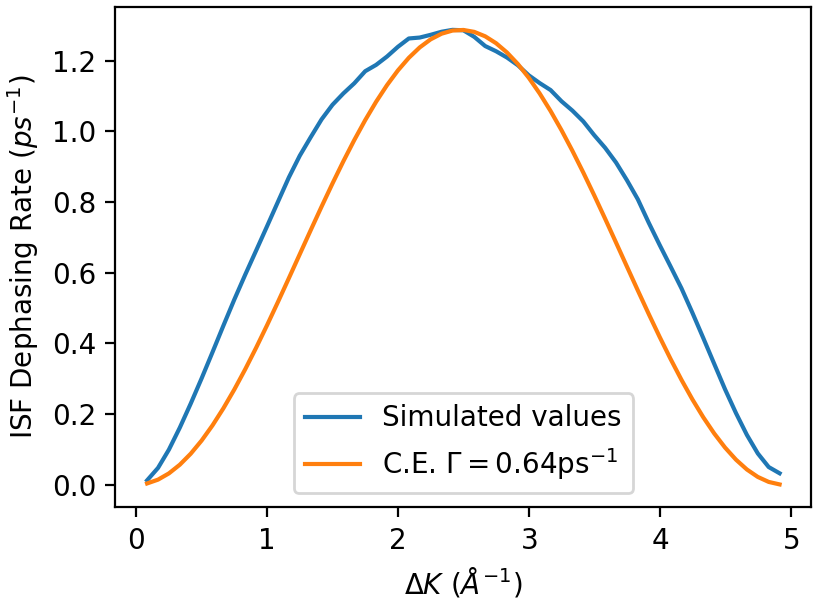
\includegraphics[width=1.0\textwidth]{alpha_deltak}
		\caption{The dephasing rate of the ISF as a function of $\left|\Delta{\vec{K}}\right|$ in the $\left[1\bar{1}0\right]$ direction alongside the theoretical form predicted by the Chudley-Elliot idealized hopping model \cite{Chudley_1961} at a rate of $\SI{0.64}{\per\pico\second}$.}
		\label{fig:alpha_deltak}
	\end{subfigure}
	\hfill	
	\begin{subfigure}{0.49\textwidth}
		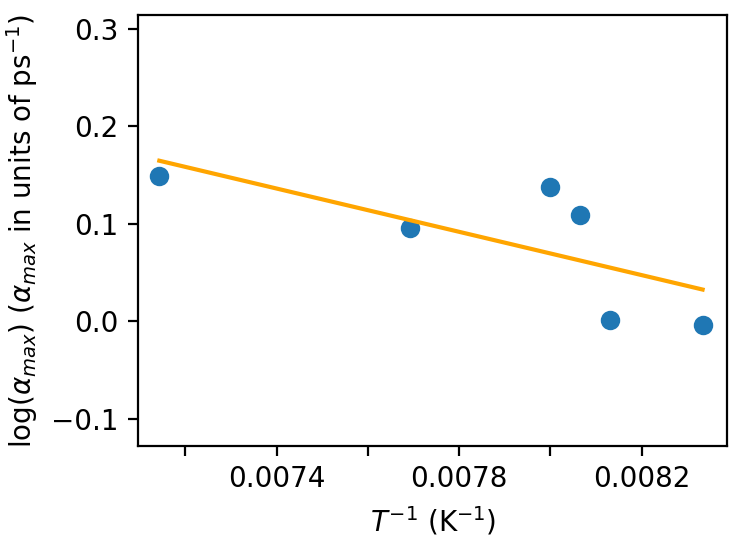
\includegraphics[width=1.0\textwidth]{ahrrenius_plot}
		\caption{Logarithm of the maximum ISF dephasing rate (proportional to the hopping rate) as a function of inverse temperature between $\SI{120}{\kelvin}$ and $\SI{140}{\kelvin}$. The linear fit suggests that the hopping process follows an Arrhenius law with activation energy $9.6\pm \SI{1.5}{\mev}$. The pre-exponential factor (y-cut on this plot) differs from the experimentally determined value.}
		\label{fig:ahrrenius_plot}
	\end{subfigure}

	\caption{Analysis of the hopping rate and activation energy of the molecular dynamics simulation.}	
\end{figure}

\chapter{Results of the GLE Simulations and Comparison with MD Simulations}

This chapter reports the results of GLE simulations performed on the parameter scales implied by the 3D MD simulations described in the previous chapter. The $\SI{7.4}{\tera\hertz}$ copper phonon cutoff frequency (Figure \ref{fig:phonon_dispersion_plot}) and energy auto-correlation decay rate of $\SI{1.32}{\per\pico\second}$ (Figure \ref{fig:md_kinetic_energy_autocorrelation}) inspired the investigation of $\tau$ on the order of $\frac{1}{f_{\text{cutoff}}} \sim \SI{e-1}{\pico\second}$ and $\eta \sim \SI{1}{\per\pico\second}$.

\section{Numerical Integrators and the Thermalisation of the GLE in a Background Potential} \label{sec:thermalization}

The use of velocity Verlet integration and the assumptions of the GLE in the presence of a background potential were evaluated using four background potentials:
\begin{itemize}
  \item No potential background
  \item A harmonic well
  \item A quartic well
  \item The corrugated potential extracted in Section \ref{sec:extract_potential}.
\end{itemize}
Each potential was simulated using three different integrator and memory kernel setups:
\begin{itemize}
	\item A velocity Verlet integrator with $\tau=\SI{0}{\ps}$
	\item A `modified' velocity Verlet integrator proposed in \cite{gronbech2013simple} with $\tau=\SI{0}{\ps}$
	\item A velocity Verlet integrator with $\tau=\SI{0.1}{\ps}$.
\end{itemize}
Each simulation was configured to run at $\SI{140}{\kelvin}$ assuming the fluctuation dissipation relation \ref{eq:tdomain_corr} holds. Each configuration was run $1000$ times for $\SI{500}{\pico\second}$ and the mean temperature of each run was recorded using $T=\frac{1}{k_B}\left<E_k\right>$. The results of these simulations are presented in Figure \ref{fig:thermalization_results}. The results demonstrate that the simulations with $\tau > 0$ exhibit more variance in general and all configurations had issues thermalizing with the corrugated potential. This suggests that either the fluctuation dissipation relation \ref{eq:tdomain_corr} does not hold for general background potentials or that the interplay between Velocity Verlet integrators and the GLE in a highly non-linear background force cause the simulation to exhibit a slightly incorrect temperature. In the GLE simulations which follow, small temperature adjustments were made to counteract this effect when appropriate. 

\begin{figure}
	\makebox[\textwidth][c]{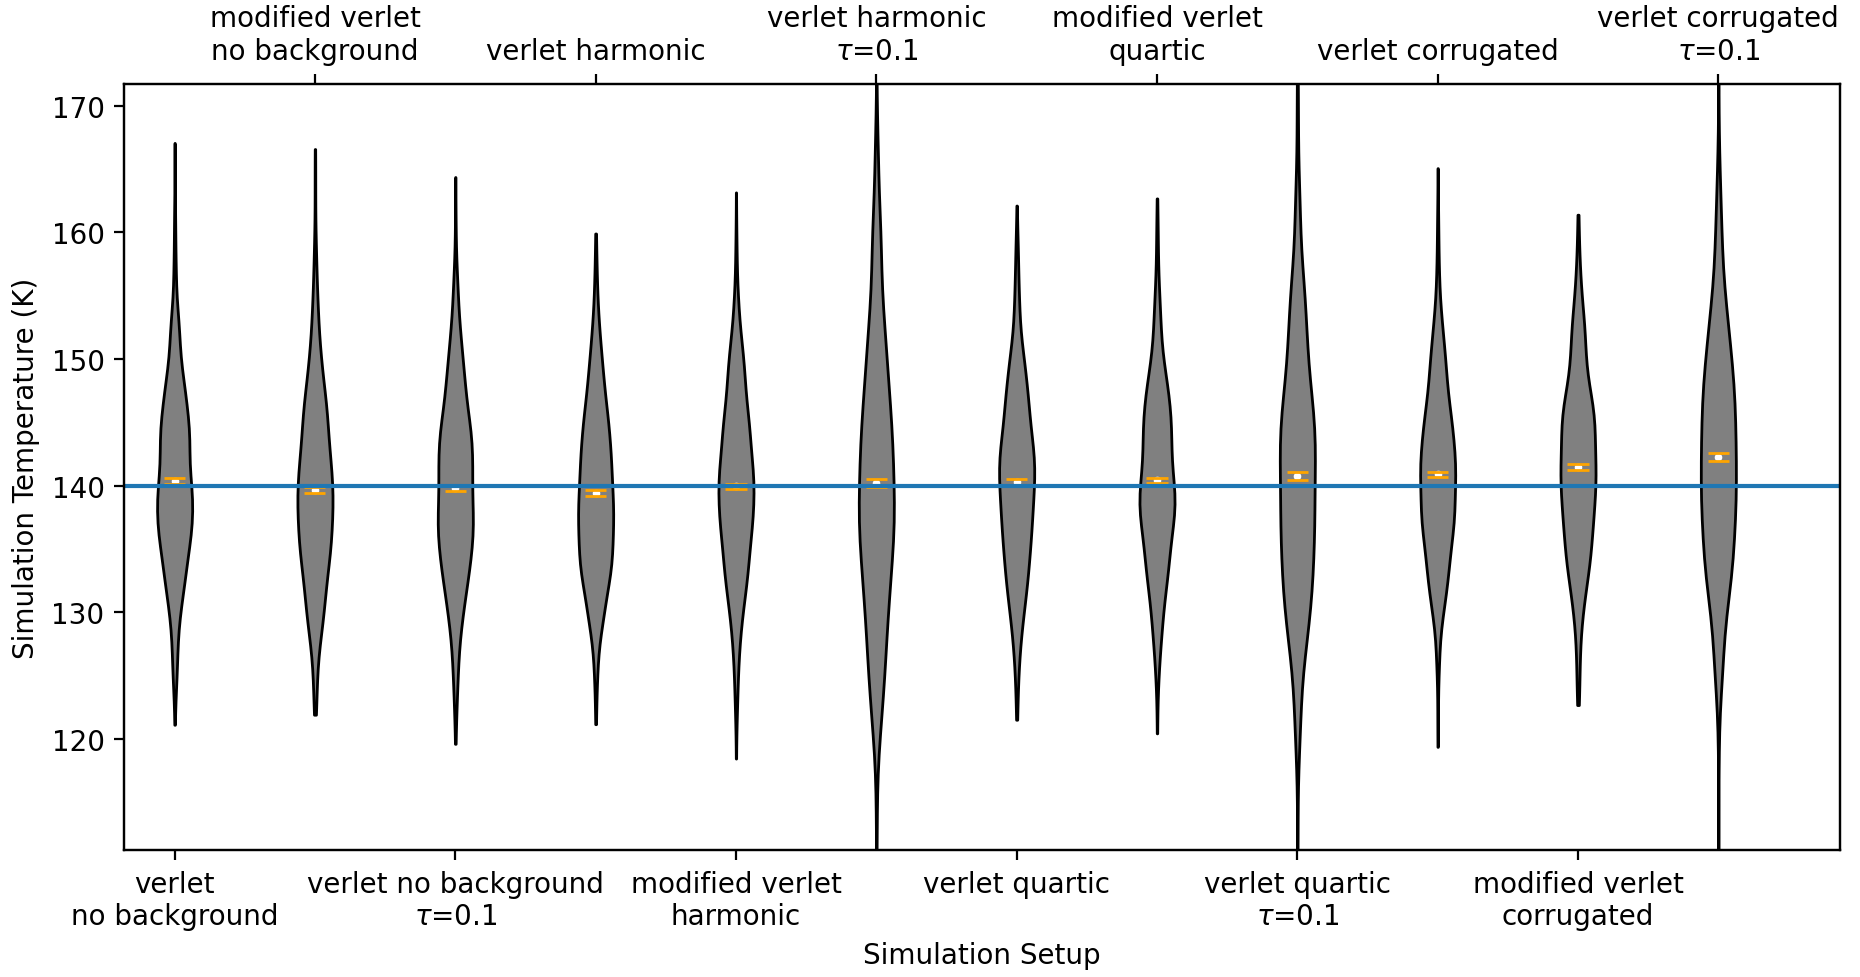
\includegraphics[width=1.2\textwidth]{gle_thermalization}}
	\caption{Distributions of the simulated temperature of various GLE simulation setups. Each configuration was run $1000$ times using the fluctuation-dissipation relation \ref{eq:tdomain_corr} at $\SI{140}{\kelvin}$ for $\SI{500}{\pico\second}$. Kernel density plots are vertically oriented showing the distribution of a single simulation temperature sample. White points indicate the mean value of a configuration and the small orange lines indicate a $\mu \pm 1\bar{\sigma}$ interval of the sample mean standard deviation $\bar{\sigma}=\frac{\sigma}{\sqrt{1000}}$.}
	\label{fig:thermalization_results}
\end{figure}

\section{Effects of the GLE Parameters on Simulated ISFs}

\begin{figure}
	\begin{subfigure}{1.0\textwidth}
		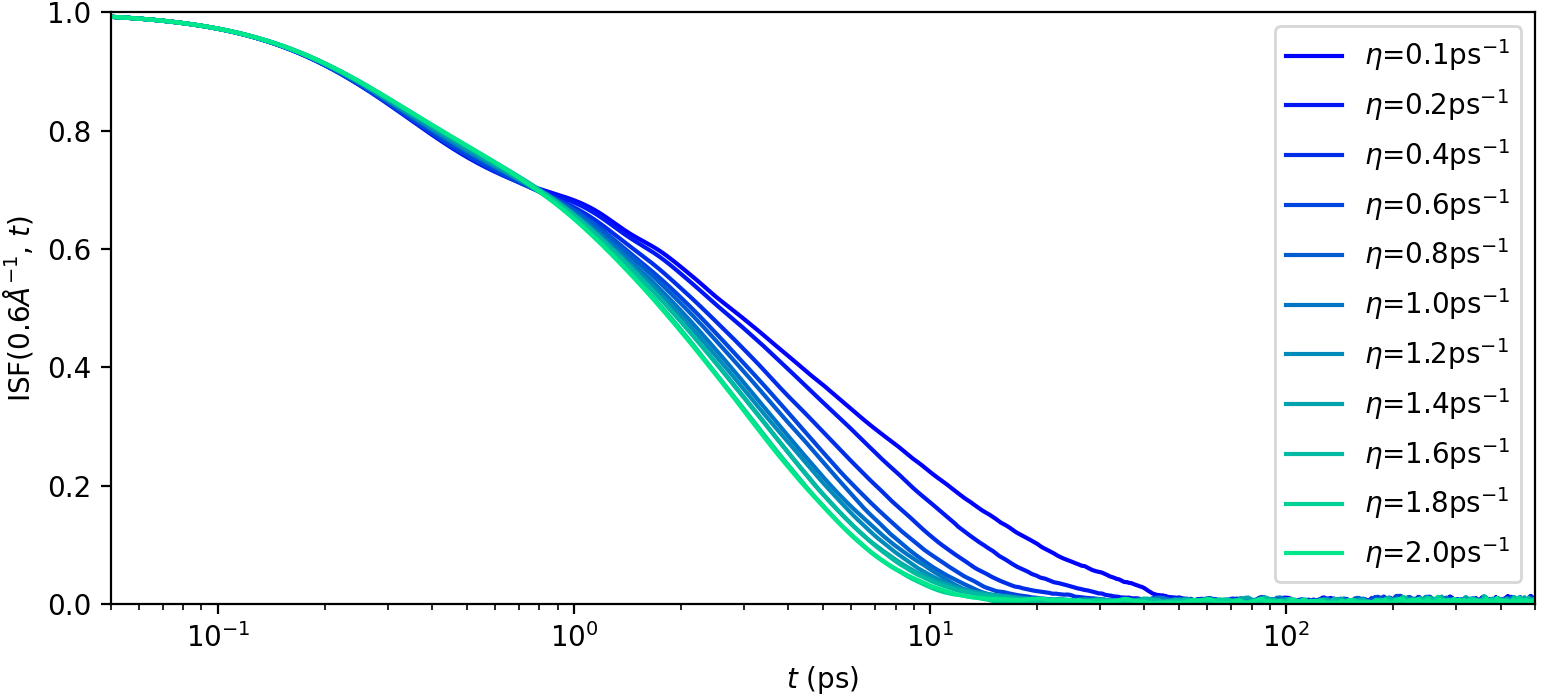
\includegraphics[width=1.0\textwidth]{vary_eta_0.6}
		\caption{ISFs on a log x-scale across a range of $\eta$ values for fixed $\tau=\SI{0.1}{\ps}$.}
		\label{fig:vary_eta_0.6}
	\end{subfigure}	
	\begin{subfigure}{0.49\textwidth}
		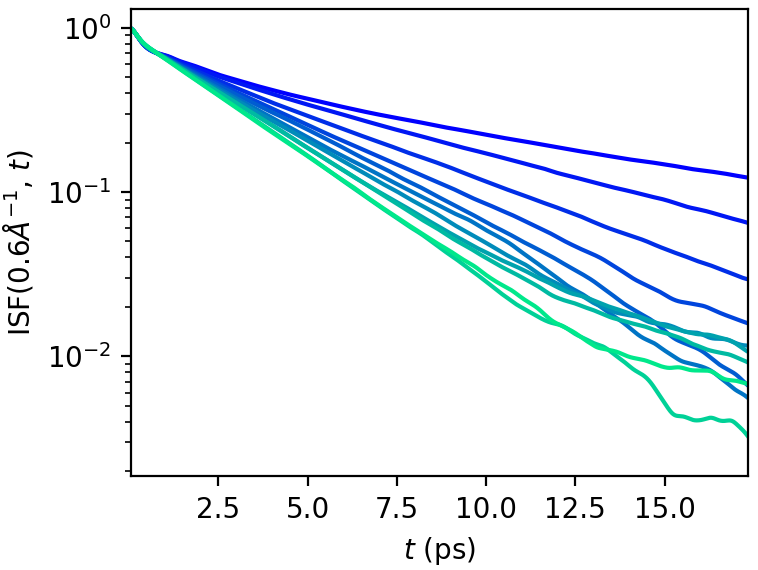
\includegraphics[width=1.0\textwidth]{vary_eta_0.6_log}
		\caption{ISFs on a log y-scale across a range of $\eta$ values for fixed $\tau=\SI{0.1}{\ps}$. The gradient of the straight line segments give the ISF dephasing rate. Shares a legend with Figure \ref{fig:vary_eta_0.6}.}
		\label{fig:vary_eta_0.6_log}
	\end{subfigure}
	\hfill
	\begin{subfigure}{0.49\textwidth}
		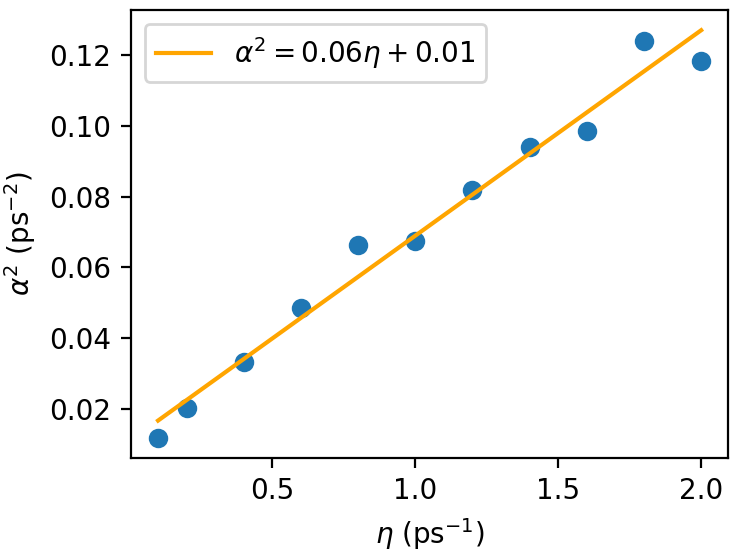
\includegraphics[width=1.0\textwidth]{alpha_vs_eta}
		\caption{The square of the dephasing rate of the ISFs in Figure \ref{fig:vary_eta_0.6} as a function of $\eta$. The form suggests a dependence of the form $\alpha \propto \sqrt{\eta}$.}
		\label{fig:alpha_vs_eta}
	\end{subfigure}
	\caption{ISFs in the $\left[1\bar{1}0\right]$ direction produced by GLE simulations using the corrugated potential obtained in Section \ref{sec:extract_potential} across a range of $\eta$ values with fixed $\tau=\SI{0.1}{\ps}$. All runs were performed at $140K$ for $\SI{100}{\ns}$ with a $\SI{1}{\fs}$ time-step.}
	\label{fig:vary_eta_all}
\end{figure}


\begin{figure}
	\begin{subfigure}{1.0\textwidth}
		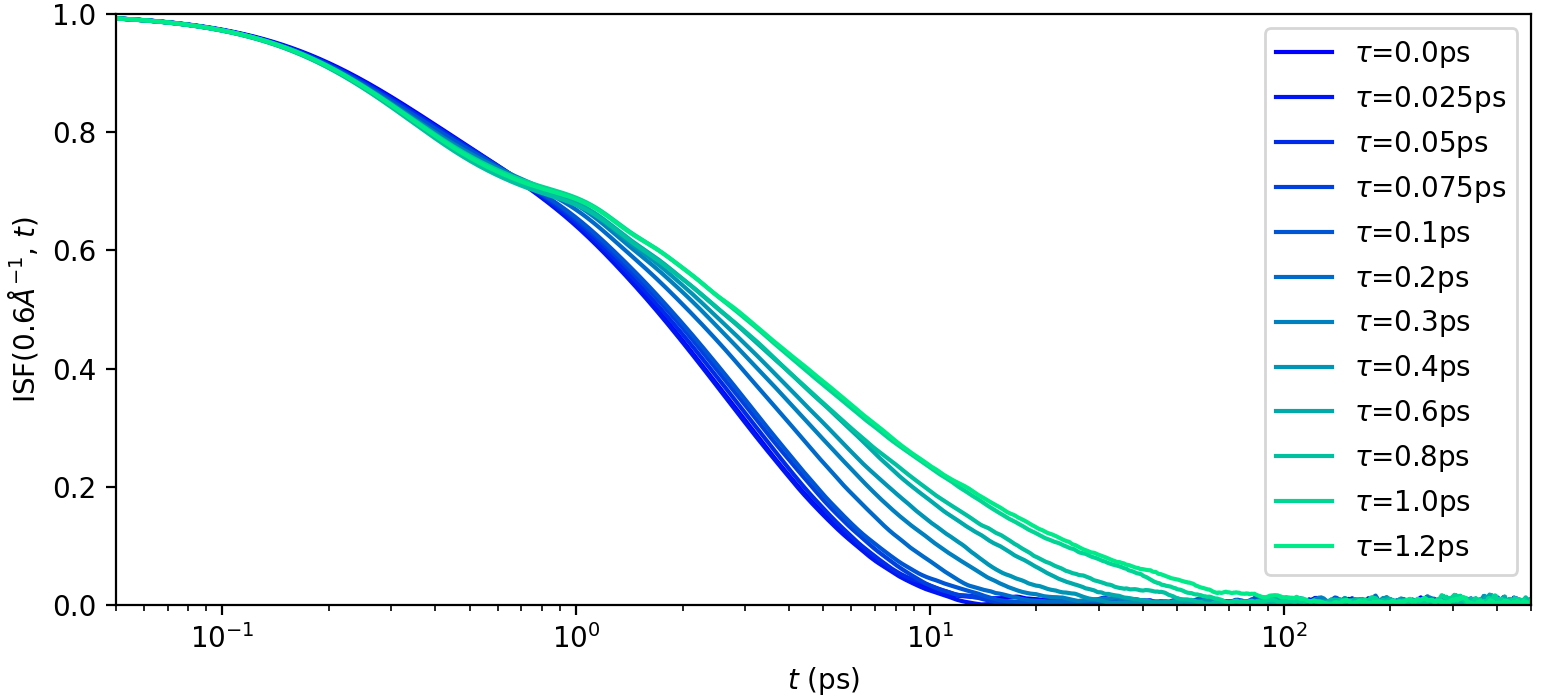
\includegraphics[width=1.0\textwidth]{vary_tau_0.6}
		\caption{ISFs on a log x-scale across a range of $\tau$ values for fixed $\eta=\SI{1.32}{\ips}$.}
		\label{fig:vary_tau_0.6}
	\end{subfigure}

	\begin{subfigure}{0.49\textwidth}
		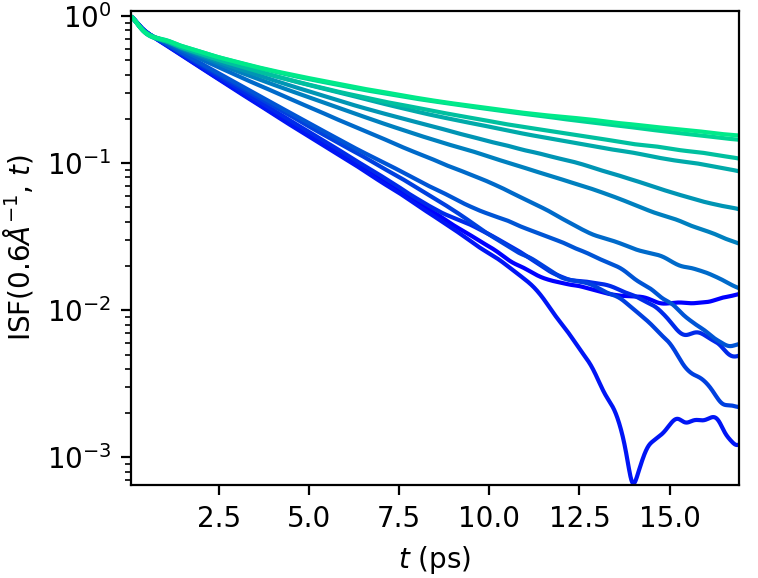
\includegraphics[width=1.0\textwidth]{vary_tau_0.6_log}
		\caption{ISFs on a log y-scale across a range of $\tau$ values for fixed $\eta=\SI{1.32}{\ips}$. The gradient of the straight line segments give the ISF dephasing rate. Shares a legend with Figure \ref{fig:vary_tau_0.6}.}
		\label{fig:vary_tau_0.6_log}
	\end{subfigure}
	\hfill	
	\begin{subfigure}{0.49\textwidth}
		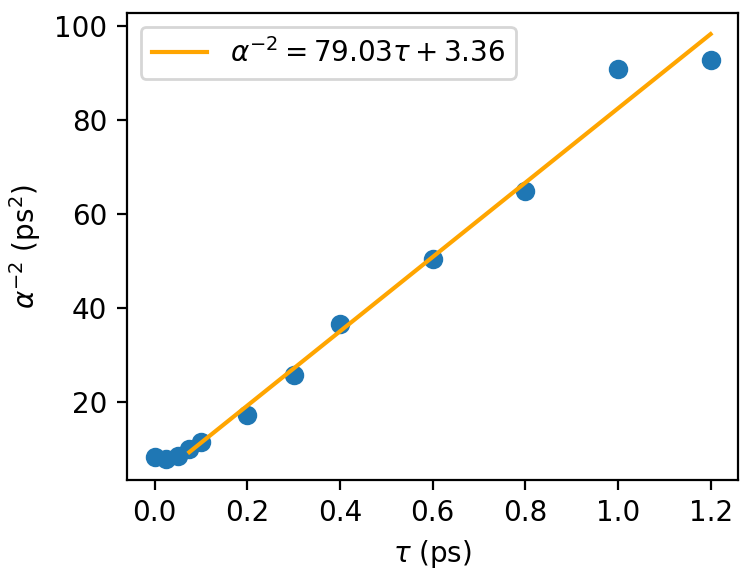
\includegraphics[width=1.0\textwidth]{alpha_vs_tau}
		\caption{The reciprocal of the dephasing rate of the ISFs in Figure \ref{fig:vary_tau_0.6} as a function of $\tau$.}
		\label{fig:alpha_vs_tau}
	\end{subfigure}
	\caption{ISFs in the $\left[1\bar{1}0\right]$ direction produced by GLE simulations using the corrugated potential obtained in Section \ref{sec:extract_potential} across a range of $\tau$ values with fixed $\eta=\SI{1.32}{\ips}$. All runs were performed at $140K$ for $\SI{100}{\ns}$ with a $\SI{1}{\fs}$ time-step.}
	\label{fig:vary_tau_all}
\end{figure}

Figures \ref{fig:vary_eta_all} \& \ref{fig:vary_tau_all} show the outcome of a number of $\SI{100}{\ns}$ GLE runs at $\SI{140}{\kelvin}$ over a range of values of $\eta$ and $\tau$.  

All runs show long term behavior of hopping between neighboring sites at a rate which varies with the value of $\tau$ and $\eta$. The effect of varying $\tau$ around $\tau=\SI{0}{\ps}$ is small as on this scale $\tau$ only affects very high frequency noise components $>\SI{10}{\thz}$ which average out on the timescale of hopping anyway. As $\tau$ increases past $\SI{e-1}{\ps}$, the simulations exhibit a slower hopping rate since $\tau$ begins to strongly suppress the frequency range which drive hopping on the timescale of $\SI{1}{\ps}$.

The hopping rate is observed to increase with the friction parameter $\eta$. This is an expected result within transition state theory \cite{BLIGAARD2008255} as $\eta$ quantifies the coupling between the noise of the system and the particle. $\eta$ thereby determines the rate at which the particle changes its energy. With no friction, the particle's total energy can never change and must therefore stay bound to its local absorption site. 

The results in Figure \ref{fig:alpha_vs_eta} \& \ref{fig:alpha_vs_tau} suggest an asymptotic relationship of the form $\alpha \propto \sqrt{\frac{\eta}{\tau}}$. While this origin of this relationship is not well understood, it is interesting to notice that within transition state theory, the pre-exponential factor of a reaction is inversely proportional to the effective mass of the system in its transition state \cite{BLIGAARD2008255}. Furthermore the GLE is introduced to model systems in which the particles driving the stochastic force are no longer of negligible mass \cite{Kubo}. It is proposed that this non-negligible mass scale affects the system's transition state effective mass linearly in $\tau$ in this parameter regime, however, this assumption is yet to be justified.   

The parameters show no effect on the ISFs at very short timescales since the thermal velocity of lithium is independent of $\eta$ and $\tau$.

\section{Comparison of ISFs Produced Using the GLE and the MD Simulation}

\begin{figure}
	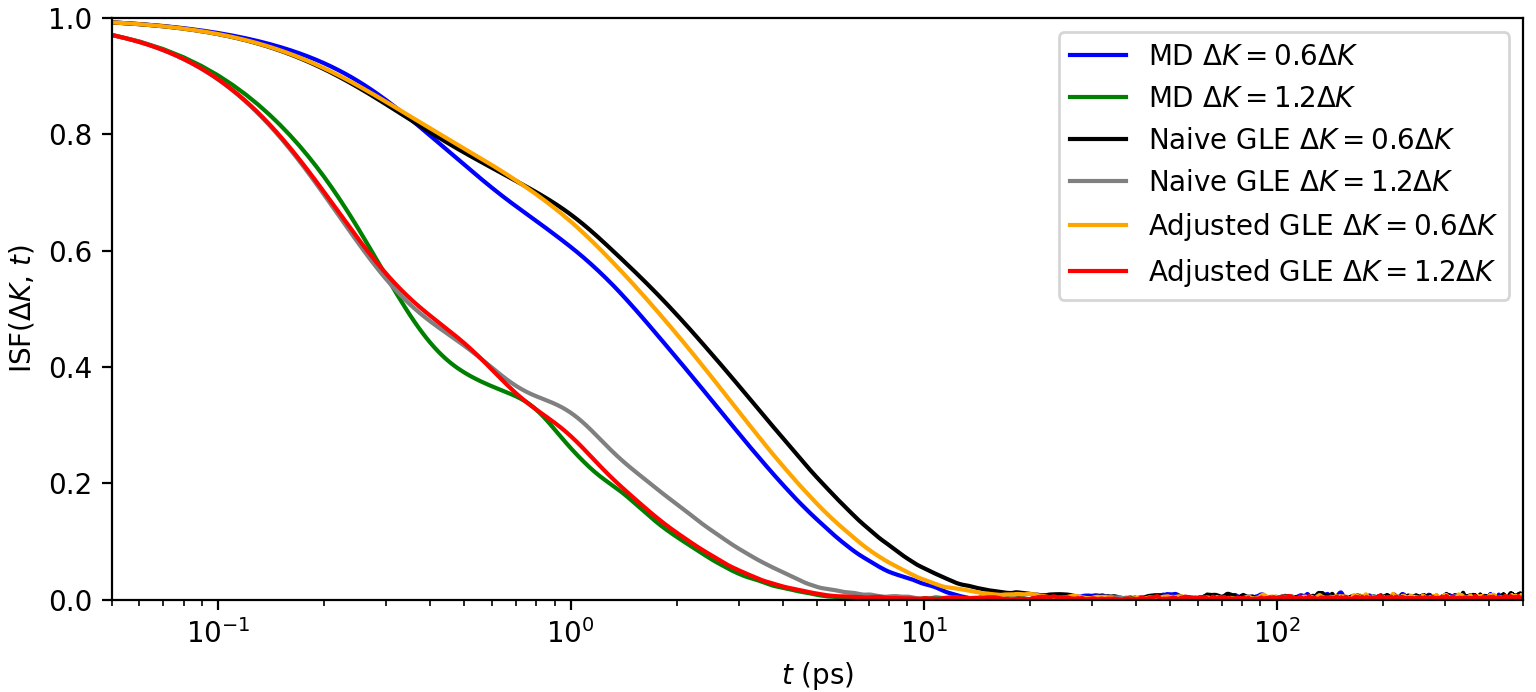
\includegraphics[width=1.0\textwidth]{md_vs_gle}
	\caption{Comparison of ISFs produced using: 1. the 3D MD simulation, 2. the GLE simulation with the naive parameter estimates $\tau=\frac{1}{f_c}=\SI{0.135}{\ps}$ and $\eta=\SI{1.32}{\ips}$ (see Figure \ref{fig:md_kinetic_energy_autocorrelation}), and 3. The GLE with parameters adjusted to $\tau=\SI{0.1}{\ps}$ and $\eta=\SI{1.9}{\ips}$ using the relationships implied by Figures \ref{fig:vary_eta_all} \& \ref{fig:vary_tau_all} to fit the MD dephasing rate.}
	\label{fig:md_vs_gle}
\end{figure}

Following the discussions in Chapter \ref{sec:gle_interpretation},  the phonon cutoff frequency, $f_c=\SI{7.4}{\thz}$, determined in Section \ref{sec:phonon_spectrum} along with the MD kinetic energy auto-correlation decay rate shown in Figure \ref{fig:md_kinetic_energy_autocorrelation} provide a `naive' estimate for reasonable GLE parameters with which to compare the GLE to the MD simulation. Figure \ref{fig:md_vs_gle} compares ISFs produced using the MD simulation to those produced with the GLE. This figure includes an additional ISF produced using the GLE parameters adjusted using the relationships in Figures \ref{fig:vary_eta_all} \& \ref{fig:vary_tau_all} to match the MD simulation's dephasing rate.

These results show that the GLE does a very good job of reproducing the ISF of the original MD simulation even when using the naive estimates presented. In particular, the dephasing rate can be exactly matched through simple adjustments of $\eta$ and $\tau$. The remaining discrepancies between the ISFs are attributed to the precise shape of the potential energy surface used in the GLE (including any errors produced in the extraction process) and differences between the noise spectrum seen in the simulation and the spectrum of the exponential memory kernel. 
